% Options for packages loaded elsewhere
\PassOptionsToPackage{unicode}{hyperref}
\PassOptionsToPackage{hyphens}{url}
%
\documentclass[
]{article}
\title{Eighth meeting notes}
\author{Daniel L.}
\date{4/08/2022}

\usepackage{amsmath,amssymb}
\usepackage{lmodern}
\usepackage{iftex}
\ifPDFTeX
  \usepackage[T1]{fontenc}
  \usepackage[utf8]{inputenc}
  \usepackage{textcomp} % provide euro and other symbols
\else % if luatex or xetex
  \usepackage{unicode-math}
  \defaultfontfeatures{Scale=MatchLowercase}
  \defaultfontfeatures[\rmfamily]{Ligatures=TeX,Scale=1}
\fi
% Use upquote if available, for straight quotes in verbatim environments
\IfFileExists{upquote.sty}{\usepackage{upquote}}{}
\IfFileExists{microtype.sty}{% use microtype if available
  \usepackage[]{microtype}
  \UseMicrotypeSet[protrusion]{basicmath} % disable protrusion for tt fonts
}{}
\makeatletter
\@ifundefined{KOMAClassName}{% if non-KOMA class
  \IfFileExists{parskip.sty}{%
    \usepackage{parskip}
  }{% else
    \setlength{\parindent}{0pt}
    \setlength{\parskip}{6pt plus 2pt minus 1pt}}
}{% if KOMA class
  \KOMAoptions{parskip=half}}
\makeatother
\usepackage{xcolor}
\IfFileExists{xurl.sty}{\usepackage{xurl}}{} % add URL line breaks if available
\IfFileExists{bookmark.sty}{\usepackage{bookmark}}{\usepackage{hyperref}}
\hypersetup{
  pdftitle={Eighth meeting notes},
  pdfauthor={Daniel L.},
  hidelinks,
  pdfcreator={LaTeX via pandoc}}
\urlstyle{same} % disable monospaced font for URLs
\usepackage[margin=1in]{geometry}
\usepackage{color}
\usepackage{fancyvrb}
\newcommand{\VerbBar}{|}
\newcommand{\VERB}{\Verb[commandchars=\\\{\}]}
\DefineVerbatimEnvironment{Highlighting}{Verbatim}{commandchars=\\\{\}}
% Add ',fontsize=\small' for more characters per line
\usepackage{framed}
\definecolor{shadecolor}{RGB}{248,248,248}
\newenvironment{Shaded}{\begin{snugshade}}{\end{snugshade}}
\newcommand{\AlertTok}[1]{\textcolor[rgb]{0.94,0.16,0.16}{#1}}
\newcommand{\AnnotationTok}[1]{\textcolor[rgb]{0.56,0.35,0.01}{\textbf{\textit{#1}}}}
\newcommand{\AttributeTok}[1]{\textcolor[rgb]{0.77,0.63,0.00}{#1}}
\newcommand{\BaseNTok}[1]{\textcolor[rgb]{0.00,0.00,0.81}{#1}}
\newcommand{\BuiltInTok}[1]{#1}
\newcommand{\CharTok}[1]{\textcolor[rgb]{0.31,0.60,0.02}{#1}}
\newcommand{\CommentTok}[1]{\textcolor[rgb]{0.56,0.35,0.01}{\textit{#1}}}
\newcommand{\CommentVarTok}[1]{\textcolor[rgb]{0.56,0.35,0.01}{\textbf{\textit{#1}}}}
\newcommand{\ConstantTok}[1]{\textcolor[rgb]{0.00,0.00,0.00}{#1}}
\newcommand{\ControlFlowTok}[1]{\textcolor[rgb]{0.13,0.29,0.53}{\textbf{#1}}}
\newcommand{\DataTypeTok}[1]{\textcolor[rgb]{0.13,0.29,0.53}{#1}}
\newcommand{\DecValTok}[1]{\textcolor[rgb]{0.00,0.00,0.81}{#1}}
\newcommand{\DocumentationTok}[1]{\textcolor[rgb]{0.56,0.35,0.01}{\textbf{\textit{#1}}}}
\newcommand{\ErrorTok}[1]{\textcolor[rgb]{0.64,0.00,0.00}{\textbf{#1}}}
\newcommand{\ExtensionTok}[1]{#1}
\newcommand{\FloatTok}[1]{\textcolor[rgb]{0.00,0.00,0.81}{#1}}
\newcommand{\FunctionTok}[1]{\textcolor[rgb]{0.00,0.00,0.00}{#1}}
\newcommand{\ImportTok}[1]{#1}
\newcommand{\InformationTok}[1]{\textcolor[rgb]{0.56,0.35,0.01}{\textbf{\textit{#1}}}}
\newcommand{\KeywordTok}[1]{\textcolor[rgb]{0.13,0.29,0.53}{\textbf{#1}}}
\newcommand{\NormalTok}[1]{#1}
\newcommand{\OperatorTok}[1]{\textcolor[rgb]{0.81,0.36,0.00}{\textbf{#1}}}
\newcommand{\OtherTok}[1]{\textcolor[rgb]{0.56,0.35,0.01}{#1}}
\newcommand{\PreprocessorTok}[1]{\textcolor[rgb]{0.56,0.35,0.01}{\textit{#1}}}
\newcommand{\RegionMarkerTok}[1]{#1}
\newcommand{\SpecialCharTok}[1]{\textcolor[rgb]{0.00,0.00,0.00}{#1}}
\newcommand{\SpecialStringTok}[1]{\textcolor[rgb]{0.31,0.60,0.02}{#1}}
\newcommand{\StringTok}[1]{\textcolor[rgb]{0.31,0.60,0.02}{#1}}
\newcommand{\VariableTok}[1]{\textcolor[rgb]{0.00,0.00,0.00}{#1}}
\newcommand{\VerbatimStringTok}[1]{\textcolor[rgb]{0.31,0.60,0.02}{#1}}
\newcommand{\WarningTok}[1]{\textcolor[rgb]{0.56,0.35,0.01}{\textbf{\textit{#1}}}}
\usepackage{graphicx}
\makeatletter
\def\maxwidth{\ifdim\Gin@nat@width>\linewidth\linewidth\else\Gin@nat@width\fi}
\def\maxheight{\ifdim\Gin@nat@height>\textheight\textheight\else\Gin@nat@height\fi}
\makeatother
% Scale images if necessary, so that they will not overflow the page
% margins by default, and it is still possible to overwrite the defaults
% using explicit options in \includegraphics[width, height, ...]{}
\setkeys{Gin}{width=\maxwidth,height=\maxheight,keepaspectratio}
% Set default figure placement to htbp
\makeatletter
\def\fps@figure{htbp}
\makeatother
\setlength{\emergencystretch}{3em} % prevent overfull lines
\providecommand{\tightlist}{%
  \setlength{\itemsep}{0pt}\setlength{\parskip}{0pt}}
\setcounter{secnumdepth}{-\maxdimen} % remove section numbering
\ifLuaTeX
  \usepackage{selnolig}  % disable illegal ligatures
\fi

\begin{document}
\maketitle

\hypertarget{to-prepare-for-this-analysis}{%
\subsection{To prepare for this
analysis:}\label{to-prepare-for-this-analysis}}

\begin{itemize}
\tightlist
\item
  Step 1: Order of differencing

  \begin{itemize}
  \tightlist
  \item
    TS plot of residuals from ARIMA(0,0,0) w/ constant in not exactly
    stationary -\textgreater{} d = 1
  \end{itemize}
\item
  Step 2: AR() or MA()
\end{itemize}

\begin{enumerate}
\def\labelenumi{\arabic{enumi}.}
\tightlist
\item
  Obtain residual from current model: ARIMA(0,1,0) w/ constant
\item
  Plot PACF of the residual
\end{enumerate}

\begin{itemize}
\tightlist
\item
  Step 3: Seasonality()
\end{itemize}

\begin{enumerate}
\def\labelenumi{\arabic{enumi}.}
\tightlist
\item
  Look at the PACF to determine AR() or MA() terms
\end{enumerate}

\begin{itemize}
\tightlist
\item
  To return the RMSE, I had to use the accuracy function from the
  fabletools package. Which meant that I had to reuse or create the
  ARIMA models in the same manner shown in the fpp3 book.
\end{itemize}

\hypertarget{creating-models-with-zoo-and-the-arima-package-from-stats}{%
\subsection{Creating models with zoo() and the arima package from
stats()}\label{creating-models-with-zoo-and-the-arima-package-from-stats}}

Here we create the ts and create the autoplot of the ts using the zoo
package

\begin{Shaded}
\begin{Highlighting}[]
\NormalTok{DSNY\_BX\_zoo\_ts }\OtherTok{\textless{}{-}} \FunctionTok{ts}\NormalTok{(DSNY\_third\_bronx[,}\SpecialCharTok{{-}}\DecValTok{1}\NormalTok{], }
                     \AttributeTok{start =} \FunctionTok{as.yearmon}\NormalTok{(DSNY\_third\_bronx}\SpecialCharTok{$}\NormalTok{month)[}\DecValTok{1}\NormalTok{], }
                     \AttributeTok{frequency =} \DecValTok{12}\NormalTok{)}

\FunctionTok{autoplot}\NormalTok{(}\FunctionTok{as.zoo}\NormalTok{(DSNY\_BX\_zoo\_ts))}
\end{Highlighting}
\end{Shaded}

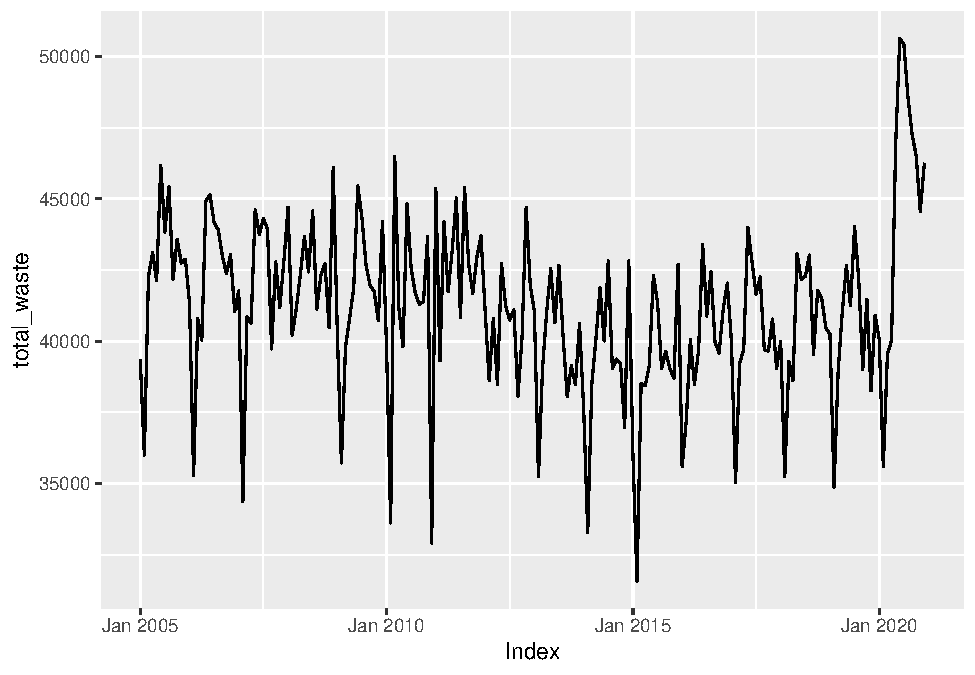
\includegraphics{eighth_meeting_notes_files/figure-latex/autoplot-1.pdf}

\hypertarget{textarima000-with-constant}{%
\subsubsection{\texorpdfstring{\(\text{ARIMA(0,0,0)}\) with
constant}{\textbackslash text\{ARIMA(0,0,0)\} with constant}}\label{textarima000-with-constant}}

\begin{Shaded}
\begin{Highlighting}[]
\NormalTok{zoo\_arima000\_fit }\OtherTok{\textless{}{-}} \FunctionTok{arima}\NormalTok{(DSNY\_BX\_zoo\_ts, }\AttributeTok{order =} \DecValTok{1} \SpecialCharTok{+} \FunctionTok{c}\NormalTok{(}\DecValTok{0}\NormalTok{,}\DecValTok{0}\NormalTok{,}\DecValTok{0}\NormalTok{))}
\CommentTok{\#names(zoo\_arima000\_fit)}
\NormalTok{res\_arima000 }\OtherTok{\textless{}{-}}\NormalTok{ zoo\_arima000\_fit}\SpecialCharTok{$}\NormalTok{residuals}
\FunctionTok{acf}\NormalTok{(res\_arima000, }\AttributeTok{lag.max =} \DecValTok{36}\NormalTok{)}
\end{Highlighting}
\end{Shaded}

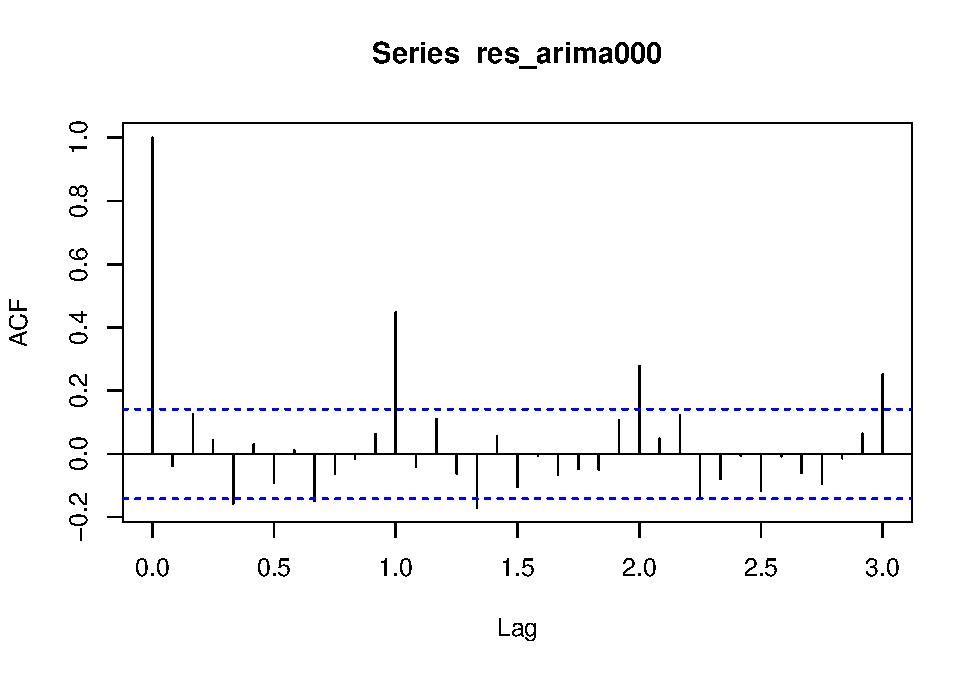
\includegraphics{eighth_meeting_notes_files/figure-latex/arima000-1.pdf}

\begin{Shaded}
\begin{Highlighting}[]
\FunctionTok{pacf}\NormalTok{(res\_arima000, }\AttributeTok{lag.max =} \DecValTok{36}\NormalTok{)}
\end{Highlighting}
\end{Shaded}

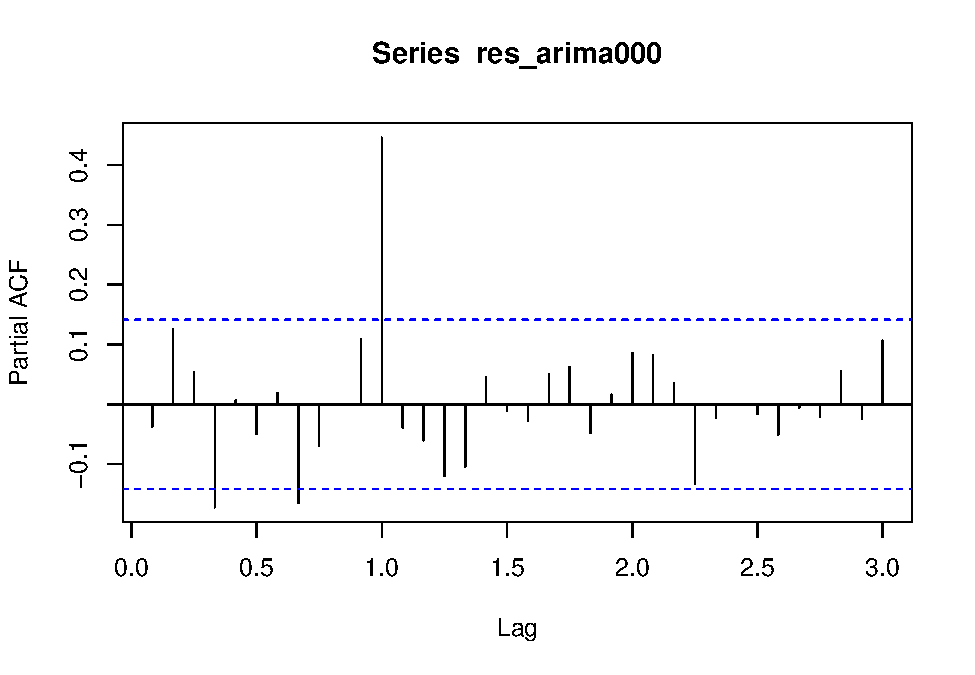
\includegraphics{eighth_meeting_notes_files/figure-latex/arima000-2.pdf}

\begin{Shaded}
\begin{Highlighting}[]
\FunctionTok{accuracy}\NormalTok{(bx\_arima000\_fit)[}\DecValTok{4}\NormalTok{]}
\end{Highlighting}
\end{Shaded}

\begin{verbatim}
## # A tibble: 1 x 1
##    RMSE
##   <dbl>
## 1 2998.
\end{verbatim}

The lags are in decimal format. With the frequency defined as 12, I
believe Lag 1.0 = 12, Lag 2.0 = 24, Lag 3.0 = 36.

For ARIMA models with differencing, the differenced series follows a
zero-mean ARMA model. Documentation by
\href{https://www.rdocumentation.org/packages/stats/versions/3.6.2/topics/arima}{DataCamp}.

\hypertarget{textarima000-with-constant-and-seasonal}{%
\subsubsection{\texorpdfstring{\(\text{ARIMA(0,0,0)}\) with constant and
seasonal}{\textbackslash text\{ARIMA(0,0,0)\} with constant and seasonal}}\label{textarima000-with-constant-and-seasonal}}

\(\text{ARIMA(0,0,0)(1,0,0)}_{12}\)

\begin{Shaded}
\begin{Highlighting}[]
\NormalTok{bx\_arima000\_fit\_cons\_seasonal }\OtherTok{\textless{}{-}}\NormalTok{ bx\_ts }\SpecialCharTok{\%\textgreater{}\%} 
  \FunctionTok{model}\NormalTok{(}\AttributeTok{arima000\_constant\_seasonal =} \FunctionTok{ARIMA}\NormalTok{(total\_waste }\SpecialCharTok{\textasciitilde{}} \DecValTok{1} \SpecialCharTok{+} 
                                     \FunctionTok{pdq}\NormalTok{(}\DecValTok{0}\NormalTok{,}\DecValTok{0}\NormalTok{,}\DecValTok{0}\NormalTok{) }\SpecialCharTok{+} 
                                     \FunctionTok{PDQ}\NormalTok{(}\DecValTok{1}\NormalTok{,}\DecValTok{0}\NormalTok{,}\DecValTok{0}\NormalTok{, }\AttributeTok{period =} \DecValTok{12}\NormalTok{)))}
        
\NormalTok{zoo\_arima000\_seasonal\_fit }\OtherTok{\textless{}{-}} \FunctionTok{arima}\NormalTok{(DSNY\_BX\_zoo\_ts, }
                          \AttributeTok{order =} \DecValTok{1} \SpecialCharTok{+} \FunctionTok{c}\NormalTok{(}\DecValTok{0}\NormalTok{,}\DecValTok{0}\NormalTok{,}\DecValTok{0}\NormalTok{),}
                          \AttributeTok{seasonal =} \FunctionTok{list}\NormalTok{(}\AttributeTok{order =} \FunctionTok{c}\NormalTok{(}\DecValTok{1}\NormalTok{,0L,0L), }\AttributeTok{period =} \DecValTok{12}\NormalTok{))}
\CommentTok{\#names(zoo\_arima000\_fit)}
\NormalTok{res\_arima000\_seasonal }\OtherTok{\textless{}{-}}\NormalTok{ zoo\_arima000\_seasonal\_fit}\SpecialCharTok{$}\NormalTok{residuals}
\FunctionTok{acf}\NormalTok{(res\_arima000\_seasonal, }\AttributeTok{lag.max =} \DecValTok{36}\NormalTok{)}
\end{Highlighting}
\end{Shaded}

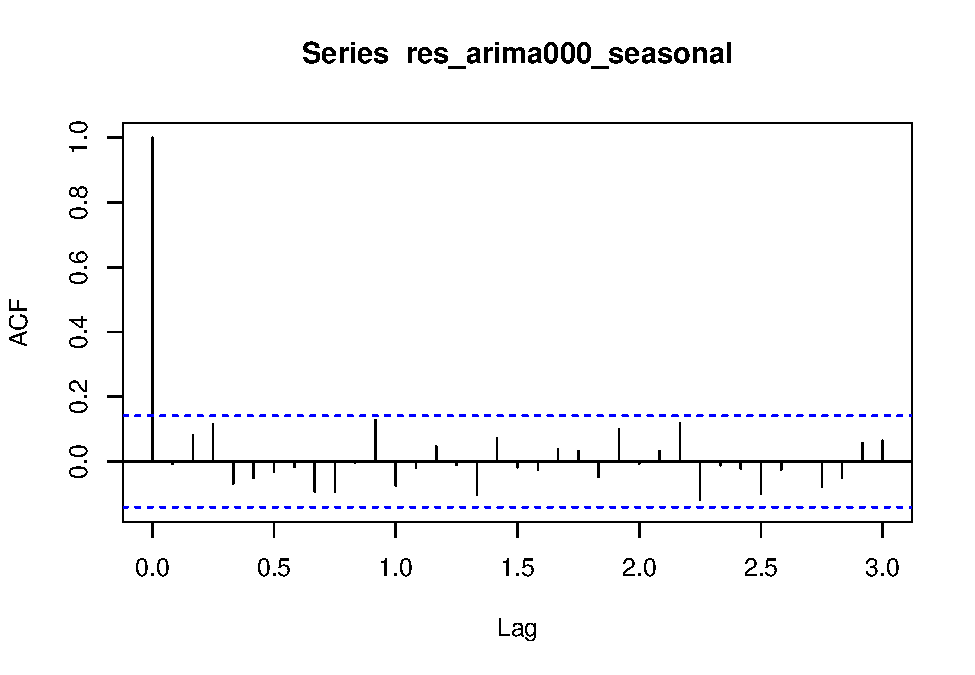
\includegraphics{eighth_meeting_notes_files/figure-latex/unnamed-chunk-3-1.pdf}

\begin{Shaded}
\begin{Highlighting}[]
\FunctionTok{pacf}\NormalTok{(res\_arima000\_seasonal, }\AttributeTok{lag.max =} \DecValTok{36}\NormalTok{)}
\end{Highlighting}
\end{Shaded}

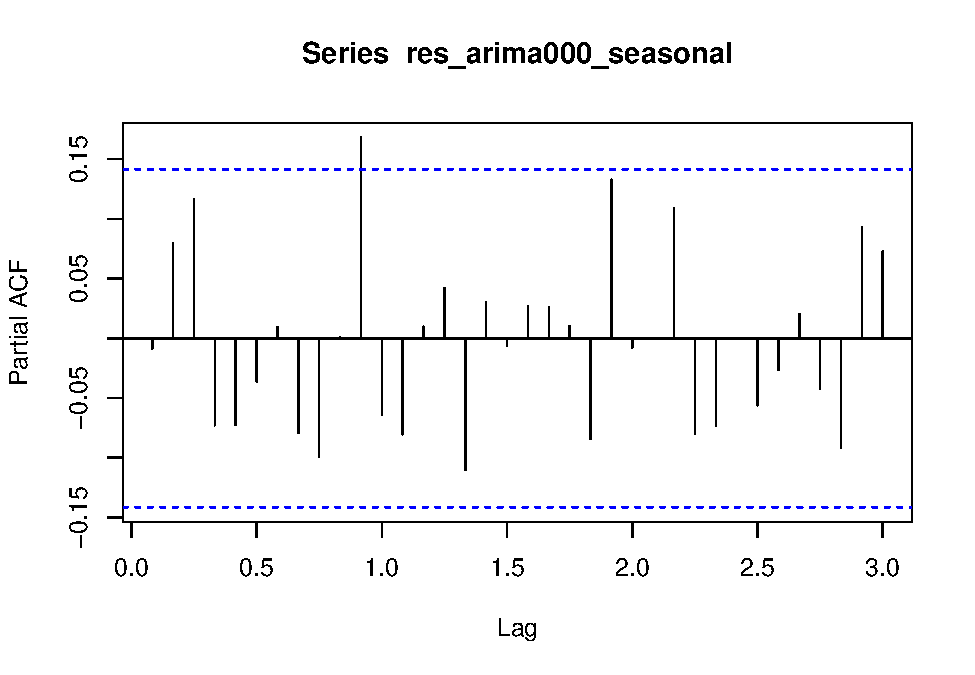
\includegraphics{eighth_meeting_notes_files/figure-latex/unnamed-chunk-3-2.pdf}

\begin{Shaded}
\begin{Highlighting}[]
\FunctionTok{accuracy}\NormalTok{(bx\_arima000\_fit\_cons\_seasonal)}
\end{Highlighting}
\end{Shaded}

\begin{verbatim}
## # A tibble: 1 x 10
##   .model                  .type    ME  RMSE   MAE    MPE  MAPE  MASE RMSSE  ACF1
##   <chr>                   <chr> <dbl> <dbl> <dbl>  <dbl> <dbl> <dbl> <dbl> <dbl>
## 1 arima000_constant_seas~ Trai~ -45.0 2482. 1755. -0.486  4.31 0.692 0.746 0.268
\end{verbatim}

\hypertarget{textarima010-with-constantmean}{%
\subsubsection{\texorpdfstring{\(\text{ARIMA(0,1,0)}\) with
constant/mean}{\textbackslash text\{ARIMA(0,1,0)\} with constant/mean}}\label{textarima010-with-constantmean}}

\begin{Shaded}
\begin{Highlighting}[]
\NormalTok{zoo\_arima010\_fit }\OtherTok{\textless{}{-}} \FunctionTok{arima}\NormalTok{(DSNY\_BX\_zoo\_ts, }
                          \AttributeTok{order =} \DecValTok{1} \SpecialCharTok{+} \FunctionTok{c}\NormalTok{(}\DecValTok{0}\NormalTok{,}\DecValTok{1}\NormalTok{,}\DecValTok{0}\NormalTok{)) }\CommentTok{\#the PACF plot return the same values}
                          \CommentTok{\#with or without the include.mean = parameter}
\NormalTok{res\_arima010 }\OtherTok{\textless{}{-}}\NormalTok{ zoo\_arima010\_fit}\SpecialCharTok{$}\NormalTok{residuals}
\FunctionTok{acf}\NormalTok{(res\_arima010, }\AttributeTok{lag.max =} \DecValTok{36}\NormalTok{)}
\end{Highlighting}
\end{Shaded}

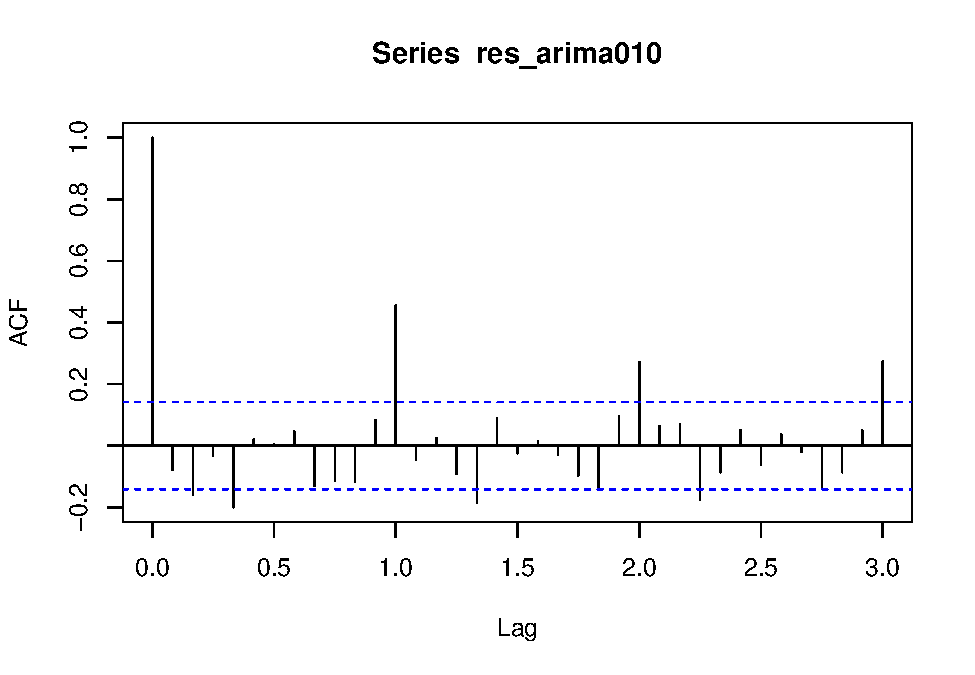
\includegraphics{eighth_meeting_notes_files/figure-latex/arima010-1.pdf}

\begin{Shaded}
\begin{Highlighting}[]
\FunctionTok{pacf}\NormalTok{(res\_arima010, }\AttributeTok{lag.max =} \DecValTok{36}\NormalTok{)}
\end{Highlighting}
\end{Shaded}

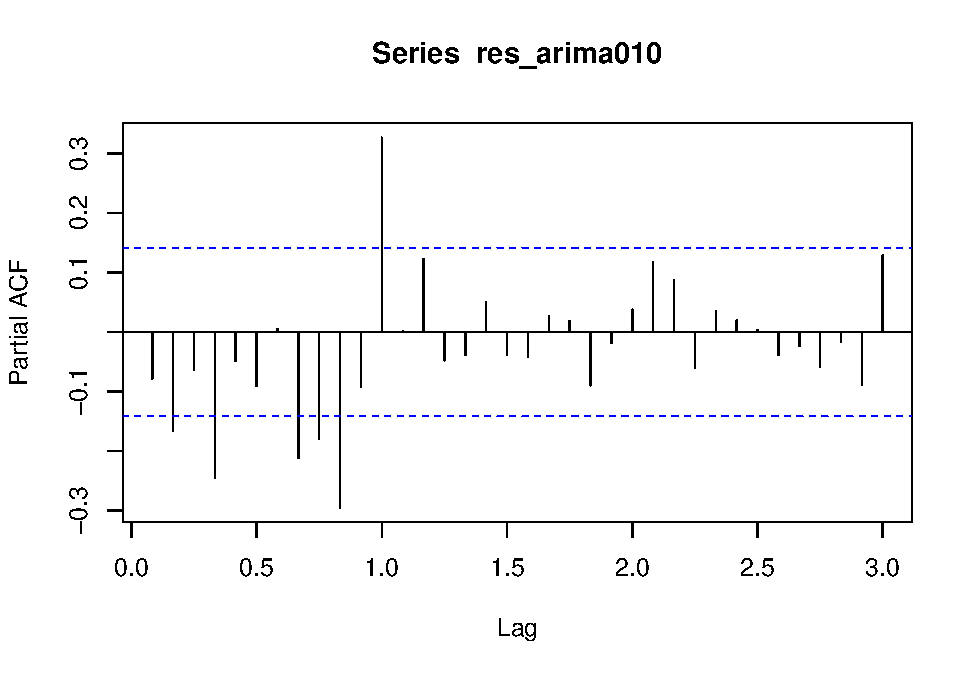
\includegraphics{eighth_meeting_notes_files/figure-latex/arima010-2.pdf}

\begin{Shaded}
\begin{Highlighting}[]
\FunctionTok{accuracy}\NormalTok{(bx\_arima010\_fit)[}\DecValTok{4}\NormalTok{]}
\end{Highlighting}
\end{Shaded}

\begin{verbatim}
## # A tibble: 1 x 1
##    RMSE
##   <dbl>
## 1 3317.
\end{verbatim}

\begin{Shaded}
\begin{Highlighting}[]
\FunctionTok{autoplot}\NormalTok{(}\FunctionTok{as.zoo}\NormalTok{(}\FunctionTok{difference}\NormalTok{(DSNY\_BX\_zoo\_ts),}\DecValTok{1}\NormalTok{))}
\end{Highlighting}
\end{Shaded}

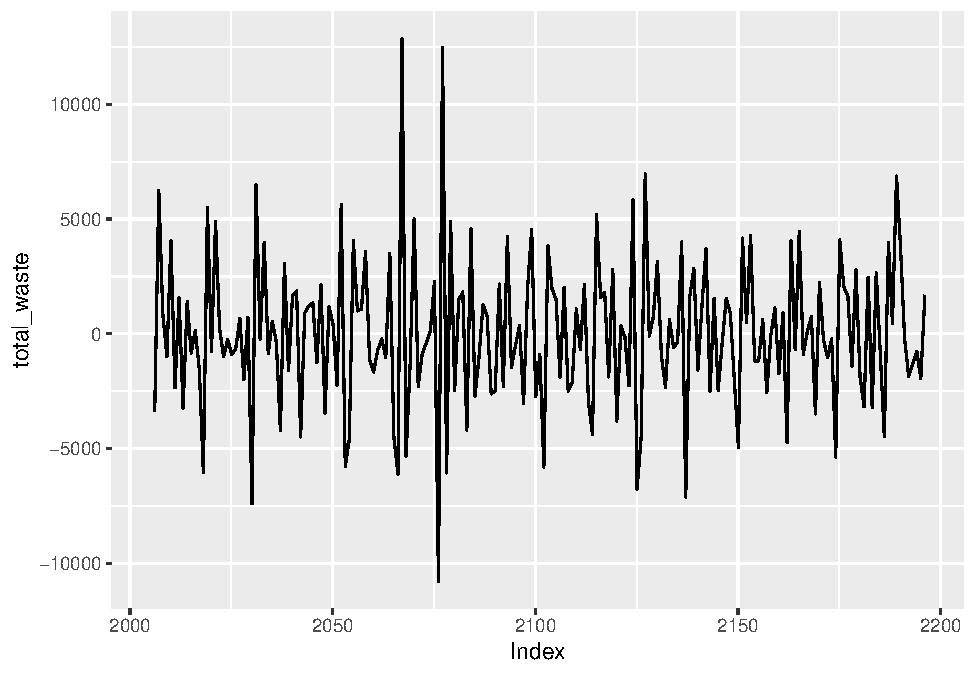
\includegraphics{eighth_meeting_notes_files/figure-latex/arima010-3.pdf}

A constant term has been added with `1 + c(0,1,0)'. As discussed before,
a negative ACF value is indicative of the need to add an MA() parameter.
Here we see that lag 3 is no longer significant, perhaps we try to add
MA(1) and MA(2) arguments to our \(\textbf{differenced}\) time series.

\hypertarget{textarima011-with-a-constant}{%
\subsubsection{\texorpdfstring{\(\text{ARIMA(0,1,1)}\) with a
constant}{\textbackslash text\{ARIMA(0,1,1)\} with a constant}}\label{textarima011-with-a-constant}}

\begin{Shaded}
\begin{Highlighting}[]
\NormalTok{bx\_arima011\_fit\_cons }\OtherTok{\textless{}{-}}\NormalTok{ bx\_ts }\SpecialCharTok{\%\textgreater{}\%} 
  \FunctionTok{model}\NormalTok{(}\AttributeTok{arima011\_constant =} \FunctionTok{ARIMA}\NormalTok{(total\_waste }\SpecialCharTok{\textasciitilde{}} \DecValTok{1} \SpecialCharTok{+} \FunctionTok{pdq}\NormalTok{(}\DecValTok{0}\NormalTok{,}\DecValTok{1}\NormalTok{,}\DecValTok{1}\NormalTok{)))}
\NormalTok{zoo\_arima011\_fit }\OtherTok{\textless{}{-}} \FunctionTok{arima}\NormalTok{(DSNY\_BX\_zoo\_ts, }
                          \AttributeTok{order =} \DecValTok{1} \SpecialCharTok{+} \FunctionTok{c}\NormalTok{(}\DecValTok{0}\NormalTok{,}\DecValTok{1}\NormalTok{,}\DecValTok{1}\NormalTok{))}
\NormalTok{res\_arima011 }\OtherTok{\textless{}{-}}\NormalTok{ zoo\_arima011\_fit}\SpecialCharTok{$}\NormalTok{residuals}
\FunctionTok{acf}\NormalTok{(res\_arima011, }\AttributeTok{lag.max =} \DecValTok{36}\NormalTok{)}
\end{Highlighting}
\end{Shaded}

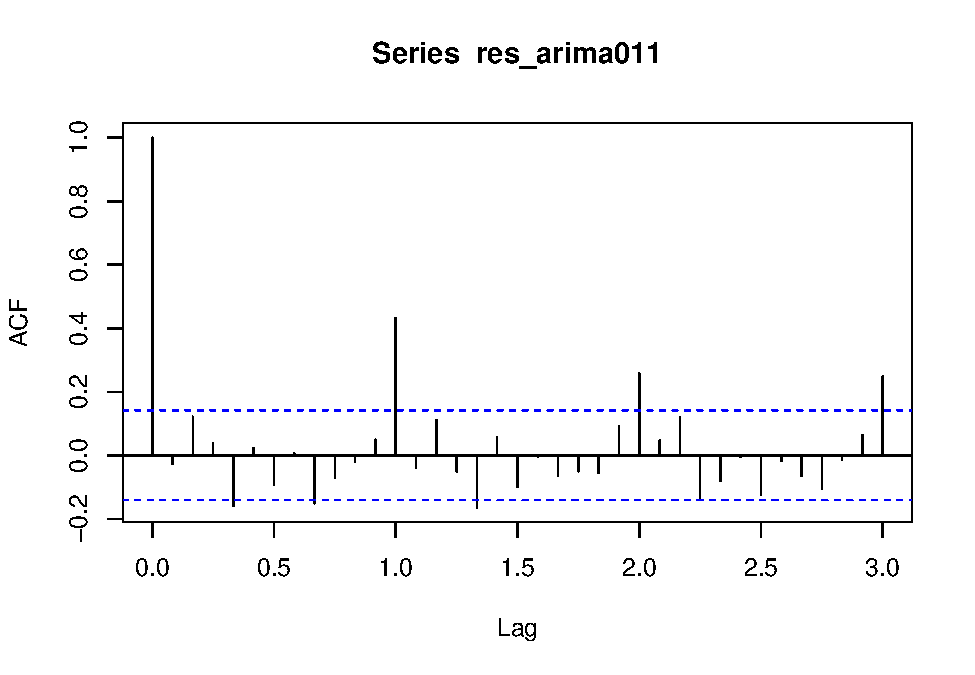
\includegraphics{eighth_meeting_notes_files/figure-latex/arima011-1.pdf}

\begin{Shaded}
\begin{Highlighting}[]
\FunctionTok{pacf}\NormalTok{(res\_arima011, }\AttributeTok{lag.max =} \DecValTok{36}\NormalTok{)}
\end{Highlighting}
\end{Shaded}

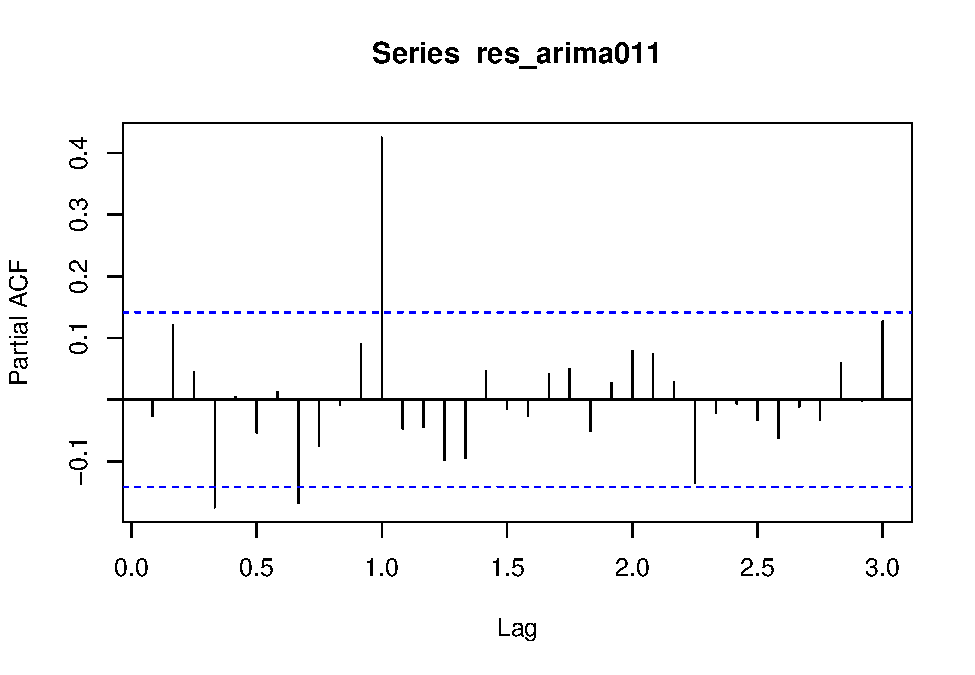
\includegraphics{eighth_meeting_notes_files/figure-latex/arima011-2.pdf}

\begin{Shaded}
\begin{Highlighting}[]
\FunctionTok{accuracy}\NormalTok{(bx\_arima011\_fit\_cons)[}\DecValTok{4}\NormalTok{]}
\end{Highlighting}
\end{Shaded}

\begin{verbatim}
## # A tibble: 1 x 1
##    RMSE
##   <dbl>
## 1 2818.
\end{verbatim}

We can see that the RMSE of this model decreased, when compared to the
ARIMA model with d = 1, and no other argument. There definitely should
be a seasonal argument, as we see a seasonal pattern of significant lags
at each integer lag.

\hypertarget{textarima012-with-a-constant}{%
\subsubsection{\texorpdfstring{\(\text{ARIMA(0,1,2)}\) with a
constant}{\textbackslash text\{ARIMA(0,1,2)\} with a constant}}\label{textarima012-with-a-constant}}

\begin{Shaded}
\begin{Highlighting}[]
\NormalTok{bx\_arima012\_cons\_fit }\OtherTok{\textless{}{-}}\NormalTok{ bx\_ts }\SpecialCharTok{\%\textgreater{}\%} 
  \FunctionTok{model}\NormalTok{(}\AttributeTok{arima012\_cons =} \FunctionTok{ARIMA}\NormalTok{(total\_waste }\SpecialCharTok{\textasciitilde{}} \DecValTok{1} \SpecialCharTok{+} \FunctionTok{pdq}\NormalTok{(}\DecValTok{0}\NormalTok{,}\DecValTok{1}\NormalTok{,}\DecValTok{2}\NormalTok{)))}

\NormalTok{zoo\_arima012\_fit }\OtherTok{\textless{}{-}} \FunctionTok{arima}\NormalTok{(DSNY\_BX\_zoo\_ts, }
                          \AttributeTok{order =} \DecValTok{1}\SpecialCharTok{+} \FunctionTok{c}\NormalTok{(}\DecValTok{0}\NormalTok{,}\DecValTok{1}\NormalTok{,}\DecValTok{2}\NormalTok{))}

\NormalTok{res\_arima012 }\OtherTok{\textless{}{-}}\NormalTok{ zoo\_arima012\_fit}\SpecialCharTok{$}\NormalTok{residuals}
\FunctionTok{acf}\NormalTok{(res\_arima012, }\AttributeTok{lag.max =} \DecValTok{36}\NormalTok{)}
\end{Highlighting}
\end{Shaded}

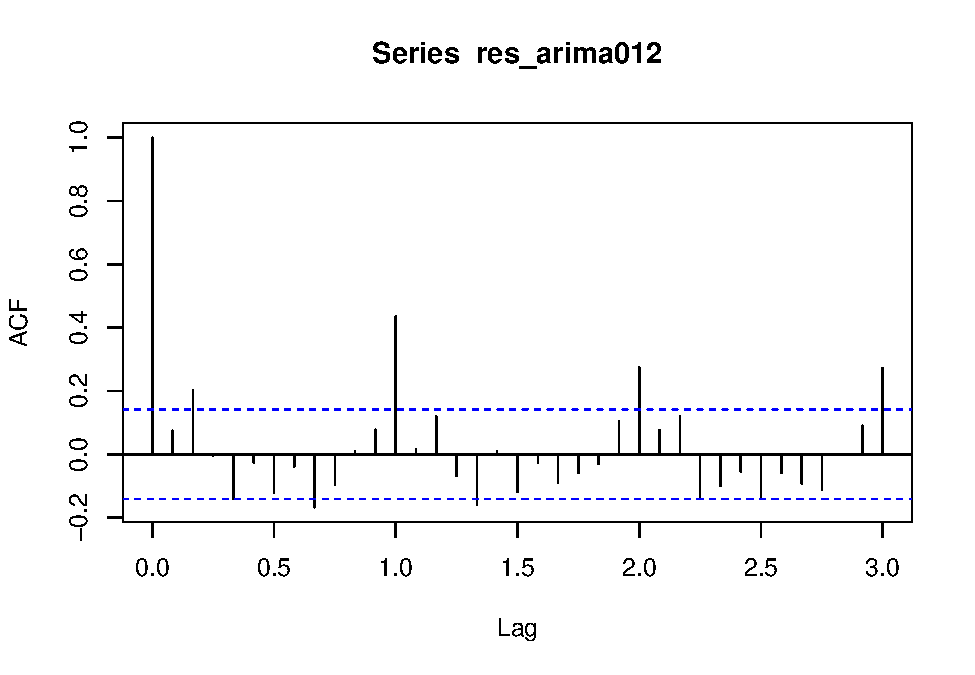
\includegraphics{eighth_meeting_notes_files/figure-latex/arima012-1.pdf}

\begin{Shaded}
\begin{Highlighting}[]
\FunctionTok{pacf}\NormalTok{(res\_arima012, }\AttributeTok{lag.max =} \DecValTok{36}\NormalTok{)}
\end{Highlighting}
\end{Shaded}

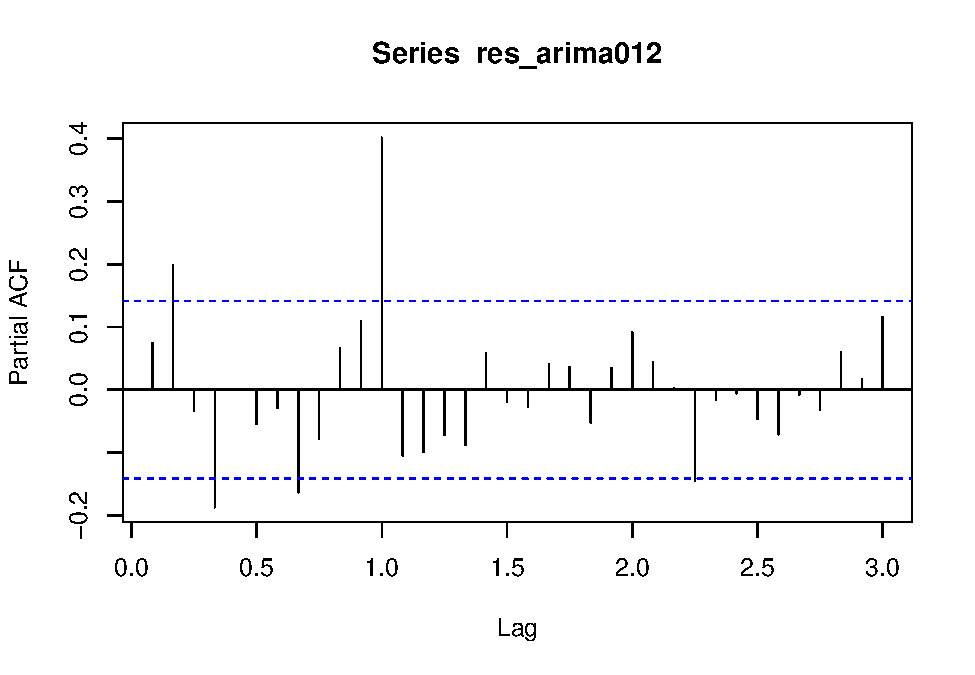
\includegraphics{eighth_meeting_notes_files/figure-latex/arima012-2.pdf}

\begin{Shaded}
\begin{Highlighting}[]
\FunctionTok{accuracy}\NormalTok{(bx\_arima012\_cons\_fit)[}\DecValTok{4}\NormalTok{]}
\end{Highlighting}
\end{Shaded}

\begin{verbatim}
## # A tibble: 1 x 1
##    RMSE
##   <dbl>
## 1 2765.
\end{verbatim}

The RMSE continues to decrease. Lags (2,4,8) are significant in the
PACF(). I am not sure if the lag 2 value of the PACF() is encouraging us
to add an AR(2) argument. I would believe that this would remove any
progress we have made. For now, I will attempt an MA(1) model. I also
think it is best to address the seasonal lags.

\hypertarget{textarima012001-with-a-constant-and-seasonal-period-12}{%
\subsubsection{\texorpdfstring{\(\text{ARIMA(0,1,2)(0,0,1)}\) with a
constant and seasonal period =
12}{\textbackslash text\{ARIMA(0,1,2)(0,0,1)\} with a constant and seasonal period = 12}}\label{textarima012001-with-a-constant-and-seasonal-period-12}}

\(\text{ARIMA(0,1,2)(0,0,1)}_{12}\)

\begin{Shaded}
\begin{Highlighting}[]
\NormalTok{bx\_arima012\_cons\_001\_12 }\OtherTok{\textless{}{-}}\NormalTok{ bx\_ts }\SpecialCharTok{\%\textgreater{}\%} 
  \FunctionTok{model}\NormalTok{(}\AttributeTok{bx\_arima012\_001\_12 =} \FunctionTok{ARIMA}\NormalTok{(total\_waste }\SpecialCharTok{\textasciitilde{}} \DecValTok{1} \SpecialCharTok{+} 
                                     \FunctionTok{pdq}\NormalTok{(}\DecValTok{0}\NormalTok{,}\DecValTok{1}\NormalTok{,}\DecValTok{2}\NormalTok{) }\SpecialCharTok{+} 
                                     \FunctionTok{PDQ}\NormalTok{(}\DecValTok{0}\NormalTok{,}\DecValTok{0}\NormalTok{,}\DecValTok{1}\NormalTok{, }\AttributeTok{period =} \DecValTok{12}\NormalTok{)))}

\NormalTok{zoo\_arima012\_001\_12fit }\OtherTok{\textless{}{-}} \FunctionTok{arima}\NormalTok{(DSNY\_BX\_zoo\_ts, }
                                \AttributeTok{order =} \DecValTok{1} \SpecialCharTok{+} \FunctionTok{c}\NormalTok{(}\DecValTok{0}\NormalTok{,}\DecValTok{1}\NormalTok{,}\DecValTok{2}\NormalTok{),}
                                \AttributeTok{seasonal =} \FunctionTok{list}\NormalTok{(}\AttributeTok{order =} \FunctionTok{c}\NormalTok{(0L,0L,}\DecValTok{1}\NormalTok{), }
                                                \AttributeTok{period =} \DecValTok{12}\NormalTok{))}

\NormalTok{res\_arima012\_001\_12 }\OtherTok{\textless{}{-}}\NormalTok{ zoo\_arima012\_001\_12fit}\SpecialCharTok{$}\NormalTok{residuals}
\FunctionTok{acf}\NormalTok{(res\_arima012\_001\_12, }\AttributeTok{lag.max =} \DecValTok{36}\NormalTok{)}
\end{Highlighting}
\end{Shaded}

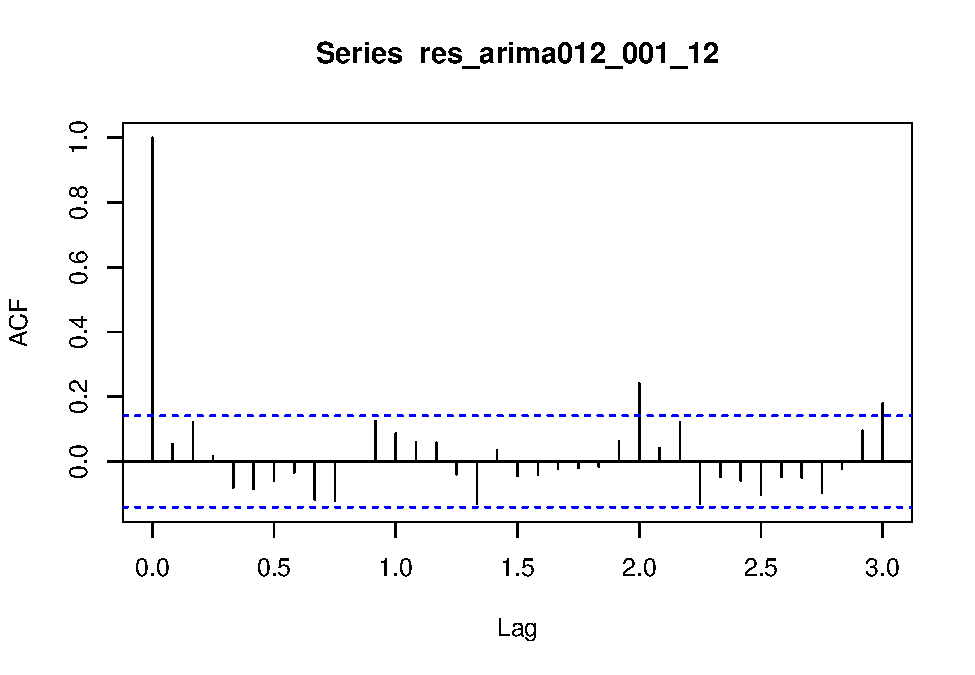
\includegraphics{eighth_meeting_notes_files/figure-latex/arima012 seasonal-1.pdf}

\begin{Shaded}
\begin{Highlighting}[]
\FunctionTok{pacf}\NormalTok{(res\_arima012\_001\_12, }\AttributeTok{lag.max =} \DecValTok{36}\NormalTok{)}
\end{Highlighting}
\end{Shaded}

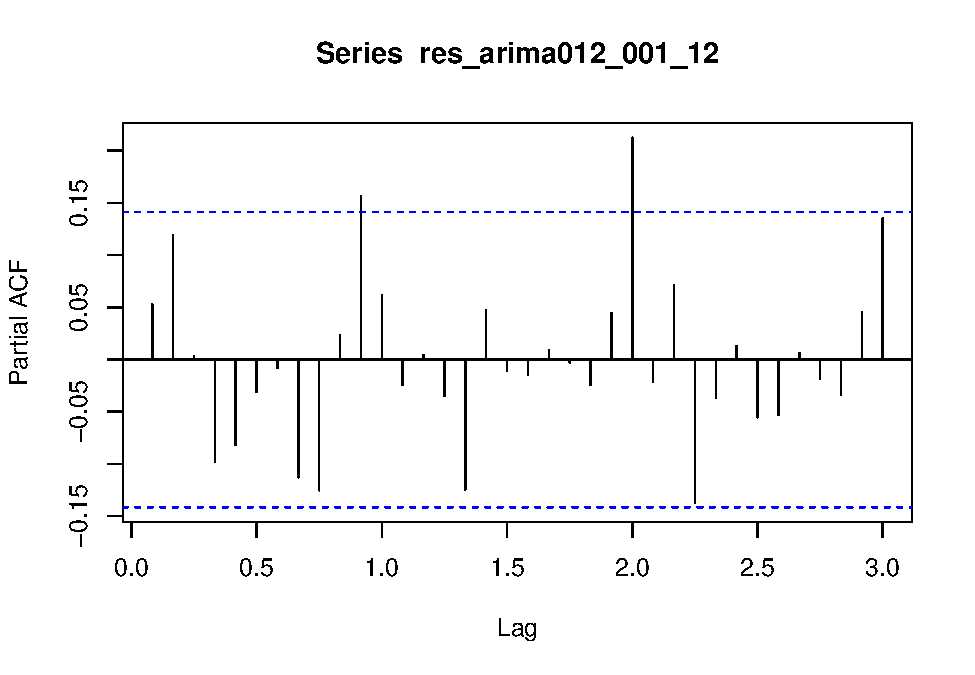
\includegraphics{eighth_meeting_notes_files/figure-latex/arima012 seasonal-2.pdf}

\begin{Shaded}
\begin{Highlighting}[]
\FunctionTok{accuracy}\NormalTok{(bx\_arima012\_cons\_001\_12)[}\DecValTok{4}\NormalTok{]}
\end{Highlighting}
\end{Shaded}

\begin{verbatim}
## # A tibble: 1 x 1
##    RMSE
##   <dbl>
## 1 2471.
\end{verbatim}

It appears that the seasonal lags in the PACF() plot appear to still be
significant. It also appears that we have bounded the PACF values
between (-0.15, 0.2). The RMSE is now the lowest of them all. From
meeting 6, I believe that this was the best ARIMA() fitting of them all.
But I will try to reduce the MA() parameter by one.

\hypertarget{textarima011001-with-a-constant-and-seasonal-period-12}{%
\subsubsection{\texorpdfstring{\(\text{ARIMA(0,1,1)(0,0,1)}\) with a
constant and seasonal period =
12}{\textbackslash text\{ARIMA(0,1,1)(0,0,1)\} with a constant and seasonal period = 12}}\label{textarima011001-with-a-constant-and-seasonal-period-12}}

\(\text{ARIMA(0,1,1)(0,0,1)}_{12}\)

\begin{Shaded}
\begin{Highlighting}[]
\NormalTok{bx\_arima011\_cons\_001\_12 }\OtherTok{\textless{}{-}}\NormalTok{ bx\_ts }\SpecialCharTok{\%\textgreater{}\%} 
  \FunctionTok{model}\NormalTok{(}\AttributeTok{bx\_arima011\_cons\_001\_12 =} \FunctionTok{ARIMA}\NormalTok{(total\_waste }\SpecialCharTok{\textasciitilde{}} \DecValTok{1} \SpecialCharTok{+} 
                                          \FunctionTok{pdq}\NormalTok{(}\DecValTok{0}\NormalTok{,}\DecValTok{1}\NormalTok{,}\DecValTok{1}\NormalTok{) }\SpecialCharTok{+} 
                                          \FunctionTok{PDQ}\NormalTok{(}\DecValTok{0}\NormalTok{,}\DecValTok{0}\NormalTok{,}\DecValTok{1}\NormalTok{, }\AttributeTok{period =} \DecValTok{12}\NormalTok{))) }

\NormalTok{zoo\_arima011\_001\_12fit }\OtherTok{\textless{}{-}} \FunctionTok{arima}\NormalTok{(DSNY\_BX\_zoo\_ts, }
                                \AttributeTok{order =} \DecValTok{1} \SpecialCharTok{+} \FunctionTok{c}\NormalTok{(}\DecValTok{0}\NormalTok{,}\DecValTok{1}\NormalTok{,}\DecValTok{1}\NormalTok{),}
                                \AttributeTok{seasonal =} \FunctionTok{list}\NormalTok{(}\AttributeTok{order =} \FunctionTok{c}\NormalTok{(0L,0L,}\DecValTok{1}\NormalTok{), }
                                                \AttributeTok{period =} \DecValTok{12}\NormalTok{))}

\NormalTok{res\_arima011\_001\_12 }\OtherTok{\textless{}{-}}\NormalTok{ zoo\_arima011\_001\_12fit}\SpecialCharTok{$}\NormalTok{residuals}
\FunctionTok{acf}\NormalTok{(res\_arima011\_001\_12, }\AttributeTok{lag.max =} \DecValTok{36}\NormalTok{)}
\end{Highlighting}
\end{Shaded}

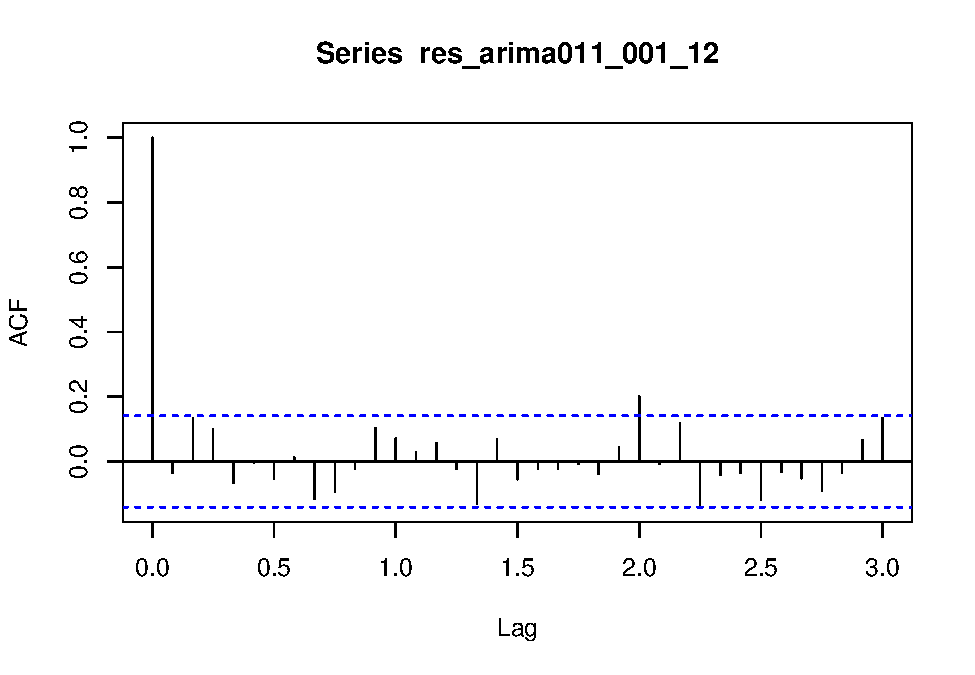
\includegraphics{eighth_meeting_notes_files/figure-latex/arima011 seasonal-1.pdf}

\begin{Shaded}
\begin{Highlighting}[]
\FunctionTok{pacf}\NormalTok{(res\_arima011\_001\_12, }\AttributeTok{lag.max =} \DecValTok{36}\NormalTok{)}
\end{Highlighting}
\end{Shaded}

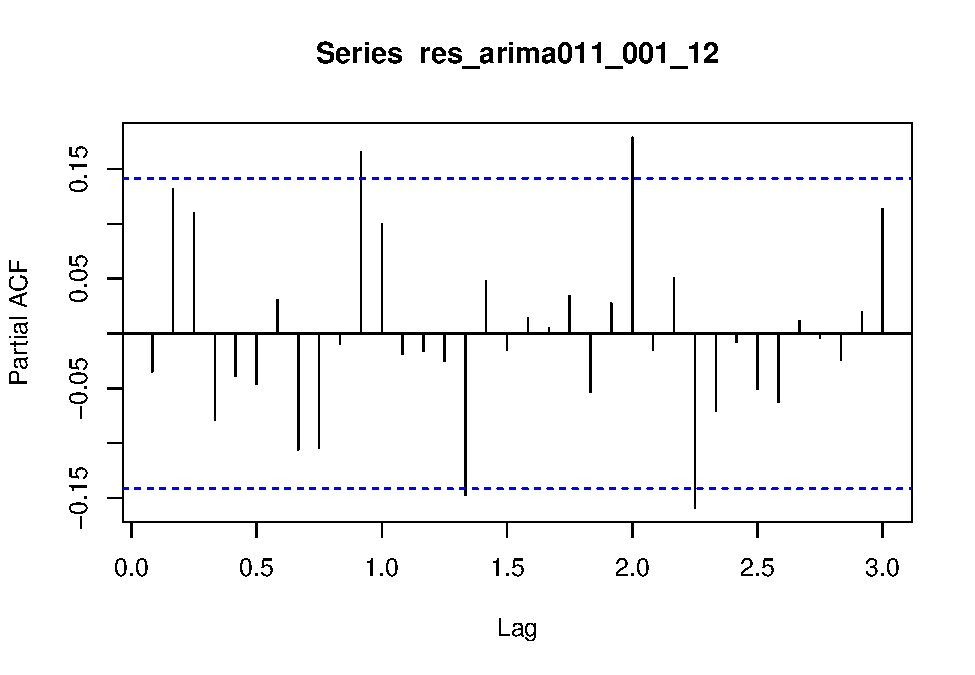
\includegraphics{eighth_meeting_notes_files/figure-latex/arima011 seasonal-2.pdf}

\begin{Shaded}
\begin{Highlighting}[]
\FunctionTok{accuracy}\NormalTok{(bx\_arima011\_cons\_001\_12)[}\DecValTok{4}\NormalTok{]}
\end{Highlighting}
\end{Shaded}

\begin{verbatim}
## # A tibble: 1 x 1
##    RMSE
##   <dbl>
## 1 2486.
\end{verbatim}

In the ACF Plot(), the seasonal lags continue to be significant, as in
they pass the 95\% threshold. A similar story with the PACF(), but the
non-seasonal lags appear to be close to the 95\% confidence levels. The
PACF values are small as well, so it would not be a major deal breaker.
With our period = 12, and seasonal lags are positive. This indicates
that it is best to add an AR() seasonal argument.

\hypertarget{textarima011100-with-a-constant-seasonal-ar-and-seasonal-period-12}{%
\subsubsection{\texorpdfstring{\(\text{ARIMA(0,1,1)(1,0,0)}\) with a
constant, seasonal AR() and seasonal period =
12}{\textbackslash text\{ARIMA(0,1,1)(1,0,0)\} with a constant, seasonal AR() and seasonal period = 12}}\label{textarima011100-with-a-constant-seasonal-ar-and-seasonal-period-12}}

\(\text{ARIMA(0,1,1)(1,0,0)}_{12}\)

\begin{Shaded}
\begin{Highlighting}[]
\NormalTok{bx\_arima011\_cons\_100\_12 }\OtherTok{\textless{}{-}}\NormalTok{ bx\_ts }\SpecialCharTok{\%\textgreater{}\%} 
  \FunctionTok{model}\NormalTok{(}\AttributeTok{bx\_arima011\_cons\_100\_12 =} \FunctionTok{ARIMA}\NormalTok{(total\_waste }\SpecialCharTok{\textasciitilde{}} \DecValTok{1} \SpecialCharTok{+} 
                                          \FunctionTok{pdq}\NormalTok{(}\DecValTok{0}\NormalTok{,}\DecValTok{1}\NormalTok{,}\DecValTok{1}\NormalTok{) }\SpecialCharTok{+} 
                                          \FunctionTok{PDQ}\NormalTok{(}\DecValTok{1}\NormalTok{,}\DecValTok{0}\NormalTok{,}\DecValTok{0}\NormalTok{, }\AttributeTok{period =} \DecValTok{12}\NormalTok{)))}

\NormalTok{zoo\_arima011\_cons\_100\_12fit }\OtherTok{\textless{}{-}} \FunctionTok{arima}\NormalTok{(DSNY\_BX\_zoo\_ts, }
                                \AttributeTok{order =} \DecValTok{1} \SpecialCharTok{+} \FunctionTok{c}\NormalTok{(}\DecValTok{0}\NormalTok{,}\DecValTok{1}\NormalTok{,}\DecValTok{1}\NormalTok{),}
                                \AttributeTok{seasonal =} \FunctionTok{list}\NormalTok{(}\AttributeTok{order =} \FunctionTok{c}\NormalTok{(}\DecValTok{1}\NormalTok{,0L,0L), }
                                                \AttributeTok{period =} \DecValTok{12}\NormalTok{))}

\NormalTok{res\_arima011\_cons\_100\_12 }\OtherTok{\textless{}{-}}\NormalTok{ zoo\_arima011\_cons\_100\_12fit}\SpecialCharTok{$}\NormalTok{residuals}
\FunctionTok{acf}\NormalTok{(res\_arima011\_cons\_100\_12, }\AttributeTok{lag.max =} \DecValTok{36}\NormalTok{)}
\end{Highlighting}
\end{Shaded}

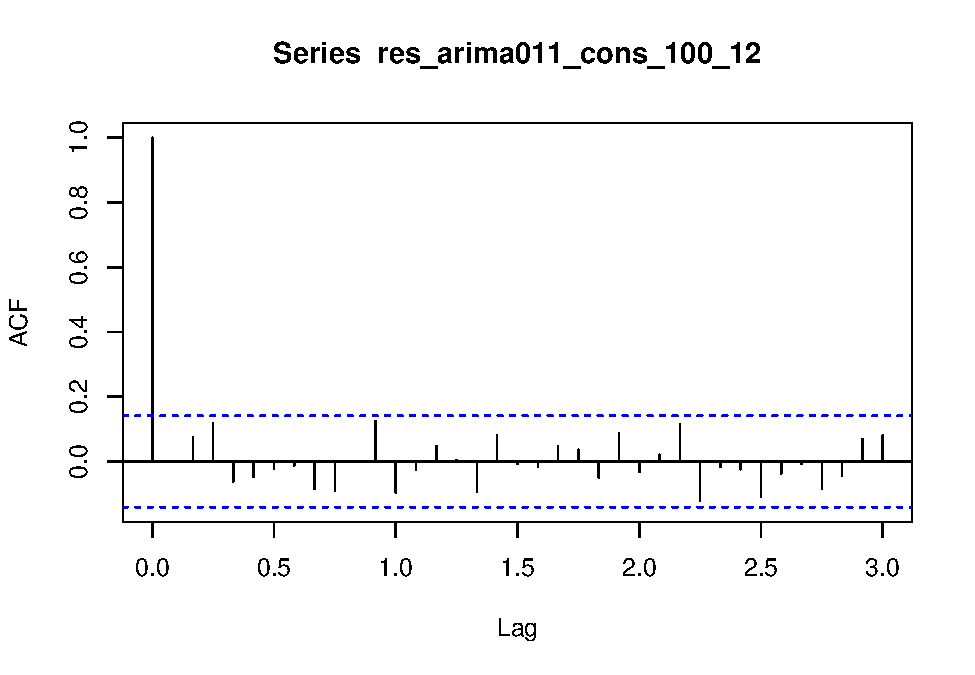
\includegraphics{eighth_meeting_notes_files/figure-latex/unnamed-chunk-4-1.pdf}

\begin{Shaded}
\begin{Highlighting}[]
\FunctionTok{pacf}\NormalTok{(res\_arima011\_cons\_100\_12, }\AttributeTok{lag.max =} \DecValTok{36}\NormalTok{)}
\end{Highlighting}
\end{Shaded}

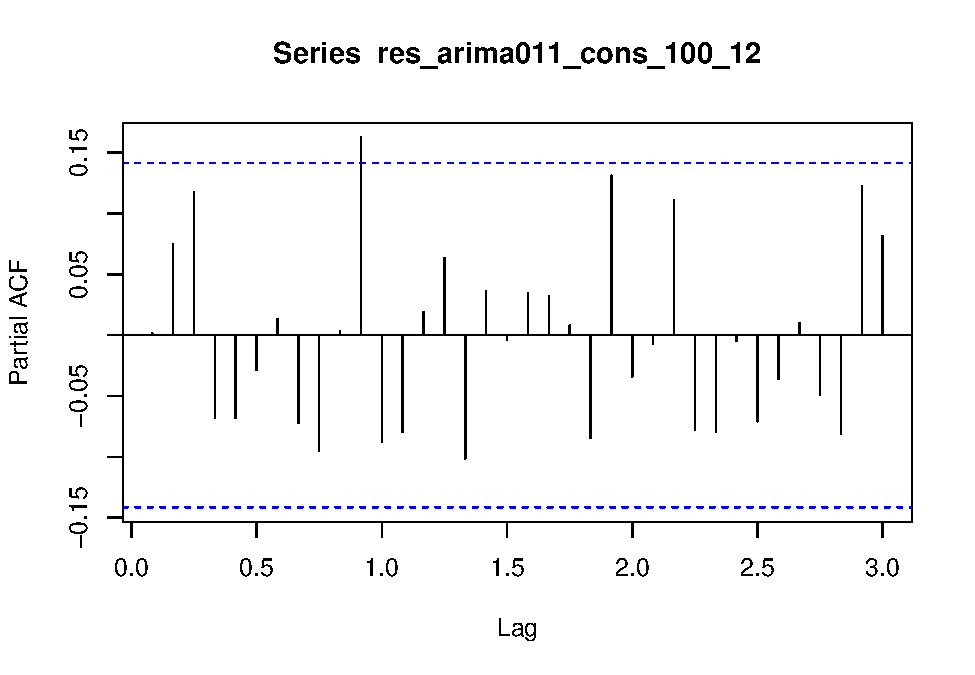
\includegraphics{eighth_meeting_notes_files/figure-latex/unnamed-chunk-4-2.pdf}

\begin{Shaded}
\begin{Highlighting}[]
\FunctionTok{accuracy}\NormalTok{(bx\_arima011\_cons\_100\_12)}
\end{Highlighting}
\end{Shaded}

\begin{verbatim}
## # A tibble: 1 x 10
##   .model                 .type    ME  RMSE   MAE    MPE  MAPE  MASE RMSSE   ACF1
##   <chr>                  <chr> <dbl> <dbl> <dbl>  <dbl> <dbl> <dbl> <dbl>  <dbl>
## 1 bx_arima011_cons_100_~ Trai~  46.2 2341. 1646. -0.202  4.05 0.649 0.704 0.0236
\end{verbatim}

This model returns the lowest RMSE. The seasonal lags in th PACF are no
longer significant. All non-seasonal lags, except for lag = 11, are
insignificant.

\hypertarget{in-conclusion}{%
\subsection{In conclusion}\label{in-conclusion}}

The models with the most promising ACF and PACF plots, and RMSE are
\(\text{ARIMA(0,1,1)(1,0,0)}_{12}\),
\(\text{ARIMA(0,0,0)(1,0,0)}_{12}\).

\end{document}
